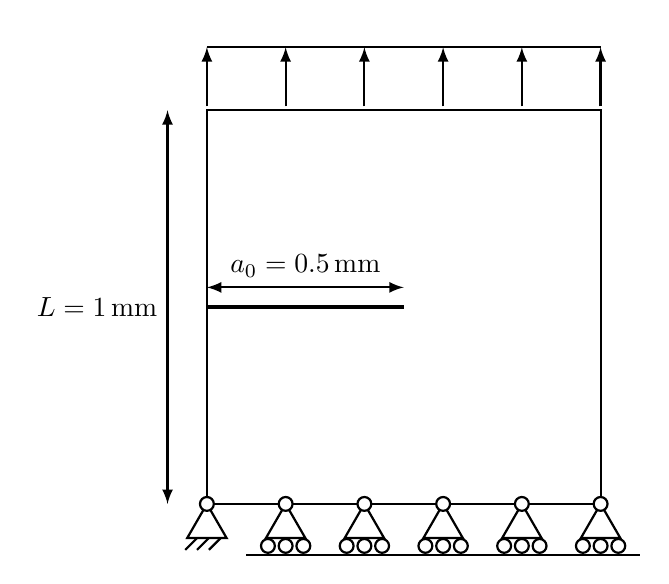
\begin{tikzpicture}[scale=5]
  % Dimensions
  \def\L{1} % Width and height of the specimen
  \def\a{0.5} % Length of the pre-crack
  
  % Specimen
  \draw[thick] (0,0) rectangle (\L,\L);

  % Pre-crack
  \draw[ultra thick] (0,\L/2) -- (\a,\L/2);
  
  % Dimensions
  \draw[thick, latex-latex] (-0.1,0) -- (-0.1,\L) node[midway, left] {$L = 1$\,mm};
  \draw[thick, latex-latex] (0,\L/2+0.05) -- (\a, \L/2+0.05) node[midway, above] {$a_0 = 0.5$\,mm};

  % Top imposed displacement
  \foreach \x in {0.0, 0.2,..., \L} {
    \draw[thick, -latex] (\x,\L+0.01) -- (\x,\L+0.16);
  }
  \draw[thick] (0,\L+0.16) -- (\L,\L+0.16) node[midway, above] {$\uimp$};

  % Lock point
  \draw[thick] (0,0) -- ({-0.1*sin(30)},{-0.1*cos(30)}) -- ({+0.1*sin(30)},{-0.1*cos(30)}) -- (0,0);
  \filldraw[thick, fill=white, draw=black] (0,0) circle (0.5pt);
  \draw[thick] ({-0.1*sin(30)+0.025},{-0.1*cos(30)}) -- ({-0.1*sin(30)-0.005},{-0.1*cos(30)-0.03});
  \draw[thick] ({-0.1*sin(30)+0.055},{-0.1*cos(30)}) -- ({-0.1*sin(30)+0.025},{-0.1*cos(30)-0.03});
  \draw[thick] ({-0.1*sin(30)+0.085},{-0.1*cos(30)}) -- ({-0.1*sin(30)+0.055},{-0.1*cos(30)-0.03});

  % Bottom block y-axis displacement
  \foreach \dx in {0.2, 0.4,...,\L} {
    \draw[thick] (\dx,0) -- ({-0.1*sin(30)+\dx},{-0.1*cos(30)}) -- ({+0.1*sin(30)+\dx},{-0.1*cos(30)}) -- (\dx,0);
    \filldraw[thick, fill=white, draw=black] (\dx,0) circle (0.5pt);
    \filldraw[thick, fill=white, draw=black] ({\dx-0.045},{-0.1*cos(30)-0.02}) circle (0.5pt);
    \filldraw[thick, fill=white, draw=black] (\dx,{-0.1*cos(30)-0.02}) circle (0.5pt);
    \filldraw[thick, fill=white, draw=black] ({\dx+0.045},{-0.1*cos(30)-0.02}) circle (0.5pt);
  }
  \draw[thick] (0.1,{-0.1*cos(30)-0.043}) -- (1.1,{-0.1*cos(30)-0.043});
\end{tikzpicture}
